% CVPR 2024 Paper Template; see https://github.com/cvpr-org/author-kit

\documentclass[10pt,twocolumn,letterpaper]{article}
\usepackage[accsupp]{axessibility}
%%%%%%%%% PAPER TYPE  - PLEASE UPDATE FOR FINAL VERSION
% \usepackage{cvpr}              % To produce the CAMERA-READY version
\usepackage[final]{cvpr}      % To produce the REVIEW version
% \usepackage[pagenumbers]{cvpr} % To force page numbers, e.g. for an arXiv version

% Import additional packages in the preamble file, before hyperref
\usepackage{graphicx}
\usepackage{color}
\usepackage{symbol}
\usepackage{placeins}
\usepackage{booktabs}
\usepackage{soul}
\usepackage{nicefrac}
\usepackage{wrapfig, tikz}
\usepackage{amsmath,amsfonts,bm,xspace}
\usepackage{bbm}
\usepackage{color}
\usepackage{enumitem, multirow}
\usepackage{fontawesome5}
\usepackage[many]{tcolorbox}
\usepackage{colortbl}


% It is strongly recommended to use hyperref, especially for the review version.
% hyperref with option pagebackref eases the reviewers' job.
% Please disable hyperref *only* if you encounter grave issues, 
% e.g. with the file validation for the camera-ready version.
%
% If you comment hyperref and then uncomment it, you should delete *.aux before re-running LaTeX.
% (Or just hit 'q' on the first LaTeX run, let it finish, and you should be clear).
\definecolor{cvprblue}{rgb}{0.21,0.49,0.74}
\usepackage[pagebackref,breaklinks,colorlinks,citecolor=cvprblue]{hyperref}

%%%%%%%%% PAPER ID  - PLEASE UPDATE
\def\paperID{5} % *** Enter the Paper ID here
\def\confName{CVPRW}
\def\confYear{2024}

\usepackage{subfloat}
\usepackage{booktabs}
\usepackage{diagbox}
\usepackage{multirow}
\usepackage{multicol}
\usepackage{makecell}
\usepackage{amsmath}
\usepackage{algorithm}
\usepackage{pifont}
\newcommand{\cmark}{\ding{51}}%
\newcommand{\xmark}{\ding{55}}%
\usepackage{algpseudocode}
\usepackage{cuted}

%%%%%%%%% TITLE - PLEASE UPDATE
\title{Source-free Domain Adaptation for Video Object Detection \\
Under Adverse Image Conditions}

%%%%%%%%% AUTHORS - PLEASE UPDATE
\author{Xingguang Zhang\\
Purdue University\\
West Lafayette, In 47907, USA\\
{\tt\small zhan3275@purdue.edu}
% For a paper whose authors are all at the same institution,
% omit the following lines up until the closing ``}''.
% Additional authors and addresses can be added with ``\and'',
% just like the second author.
% To save space, use either the email address or home page, not both
\and
Chih-Hsien Chou\\
Futurewei Technologies, Inc.\\
Santa Clara CA 95050, USA\\
{\tt\small cchou@futurewei.com}
}

\begin{document}
\maketitle
\begin{abstract}
Inverse graphics -- the task of \textit{inverting} an image into physical variables that, when rendered, enable reproduction of the observed scene -- is a fundamental challenge in computer vision and graphics.
Disentangling an image into its constituent elements, such as the shape, color, and material properties of the objects of the 3D scene that produced it, requires a comprehensive understanding of the environment.
This requirement limits the ability of existing carefully engineered approaches to generalize across domains.
Inspired by the zero-shot ability of large language models (LLMs) to generalize to novel contexts, we investigate the possibility of leveraging the broad world knowledge encoded in such models in solving inverse-graphics problems.
To this end, we propose the Inverse-Graphics Large Language Model (\mbox{\textit{IG-LLM}}), an inverse-graphics framework centered around an LLM, that autoregressively decodes a visual embedding into a structured, compositional 3D-scene representation.
We incorporate a frozen pre-trained visual encoder and a continuous numeric head to enable end-to-end training.
Through our investigation, we demonstrate the potential of LLMs to facilitate inverse graphics through next-token prediction, without the use of image-space supervision.
Our analysis opens up new possibilities for precise spatial reasoning about images that exploit the visual knowledge of LLMs.
We will release our code and data to ensure the reproducibility of our investigation and to facilitate future research at \hbox{\url{https://ig-llm.is.tue.mpg.de/}}
\end{abstract}    
\section{Introduction}

\label{sec:intro}

Reconstructing a 3D scene from video is one of the most fundamental problems in vision and has been studied for over five decades.
Today, essentially all state-of-the-art approaches are built on top of Structure-from-Motion (SfM) methods like COLMAP~\cite{schonberger2016structure}. These approaches extract sparse correspondences across frames, match them, discard outliers, and then optimize the correspondences' 3D positions alongside the camera parameters by minimizing reprojection error~\cite{schonberger2016structure}.

This framework has delivered excellent results which underlie many present-day vision applications, and so it is unsurprising that SfM systems have remained largely unchanged in the age of deep learning, save for deep-learning-based correspondence matching \cite{sarlin2020superglue,lindenberger2023lightglue,sarlin2021pixloc,detone2018superpoint}.

However, conventional SfM has a major limitation: it is not differentiable with respect to its free variables (camera poses, camera intrinsics, and per-pixel depths).
This means that SfM acts as an isolated pre-processing step that cannot be embedded into end-to-end deep learning pipelines. 
A differentiable, self-supervised SfM method would enable neural networks to be trained self-supervised on internet-scale data for a broad class of multi-view geometry problems.
This would pave the way for deep-learning based 3D reconstruction and scene understanding.

\begin{figure*}[t]
    \centering
    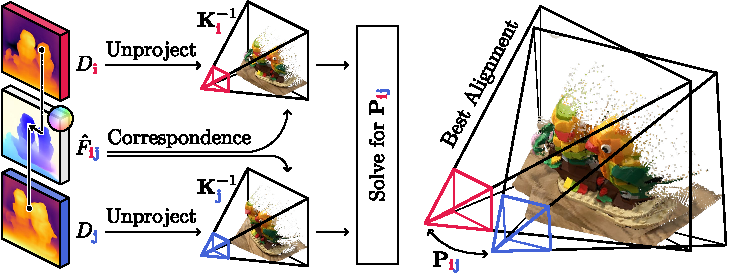
\includegraphics[width=\linewidth,]{figures/procrustes/fig_procrustes_pdf_small.pdf}
    \vspace{-12pt}
    \caption{We solve for the relative poses between consecutive frames using their depth maps, camera intrinsics, and optical flow. To do so, we first unproject their depth maps, then solve for the pose that best aligns the resulting point clouds.}
    \label{fig:procrustes}
    \vspace{-15pt}
\end{figure*}

In this paper, we present FlowMap, a differentiable and surprisingly simple camera and geometry estimation method whose outputs enable photorealistic novel view synthesis. 
FlowMap directly minimizes the difference between optical flow that is induced by a camera moving through a static 3D scene and pre-computed correspondences in the form of off-the-shelf point tracks and optical flow.
Since FlowMap is end-to-end differentiable, it can naturally be embedded in any deep learning pipeline.
Its loss is minimized only via gradient descent, leading to high-quality camera poses, camera intrinsics, and per-pixel depth.
Unlike conventional SfM, which outputs sparse 3D points that are each constrained by several views, FlowMap outputs dense per-frame depth estimates.
This is a critical advantage in downstream novel view synthesis and robotics tasks.
Unlike prior attempts at gradient-based optimization of cameras and 3D geometry~\cite{lin2021barf,nerf--,bian2022nopenerf}, we do not treat depth, intrinsics, and camera poses as free variables.
Rather, we introduce differentiable feed-forward estimates of each one: depth is parameterized via a neural network, pose is parameterized as the solution to a least-squares problem involving depth and flow, and camera intrinsics are parameterized using a differentiable selection based on optical flow consistency.
In other words, FlowMap solves SfM by learning the depth network's parameters; camera poses and intrinsics are computed via analytical feed-forward modules without free parameters of their own.
We show that this uniquely enables high-quality SfM via gradient descent while making FlowMap compatible with standard deep-learning pipelines.
Unlike recent radiance-field bundle-adjustment baselines~\cite{bian2022nopenerf,lin2021barf}, FlowMap does not use differentiable volume rendering, and so it is significantly faster to run, generally reconstructing an object-centric $360^\circ$ scan in less than 10 minutes.

Through extensive ablation studies, we show that each of FlowMap's design choices is necessary.
On popular, real-world novel view synthesis datasets (Tanks \& Temples, Mip-NeRF 360, CO3D, and LLFF), we demonstrate that FlowMap enables photo-realistic novel view synthesis up to full $360^\circ$ trajectories using Gaussian Splatting~\cite{kerbl20233d}. 
Gaussian Splats obtained from FlowMap reconstructions far outperform the state-of-the-art gradient-based bundle-adjustment method, NoPeNeRF~\cite{bian2022nopenerf}, and those obtained using the SLAM algorithm DROID-SLAM~\cite{teed2021droid}, even though both baselines require ground-truth intrinsics.
Gaussian Splats obtained from FlowMap are on par with those obtained from COLMAP~\cite{schonberger2016structure}, even though FlowMap only leverages gradient descent, is fully differentiable, and represents a complete departure from conventional SfM techniques.

\section{Related Work}\label{sec:related works}

\subsection{Link Prediction}

\noindent\textbf{Heuristic Methods.}
Heuristic-based approaches to LP compute the predefined structural features within the observed nodes and edges of the graph. 
Classic methods, such as common neighbors~\cite{adamic2003friends}, Adamic-Adar~\cite{adamic2003friends}, Jaccard coefficient~\cite{lu2011link}, and preferential attachment~\cite{barabasi1999emergence}, rely on simple heuristics that capture certain aspects of node relationships. 
Zhou \textit{et al.}~\cite{zhou2009predicting} proposed a local random walk method, whereas Jeh and Widom~\cite{jeh2002simrank} developed SimRank to quantify similarity based on the structural context. 
Although heuristic methods provide a preliminary understanding of LP, they are limited by their inability to capture complex relationships within graphs.
Furthermore, heuristic methods are effective only when the defined heuristics align with the graph structure; therefore, applying heuristic methods across all graph datasets can be challenging.


\noindent\textbf{Embedding Methods.}
Embedding methods map nodes from the graph into a low-dimensional vector space where geometric relationships mirror the graph structure. 
Koren \textit{et al.}~\cite{koren2009matrix} demonstrated the power of matrix factorization for collaborative filtering. 
Perozzi \textit{et al.}~\cite{perozzi2014deepwalk} introduced DeepWalk, using random walks to generate node sequences and employing the skip-gram model to produce embeddings. 
Tang \textit{et al.}~\cite{tang2015line} developed large-scale information network embedding (LINE), which preserves local and global structures. 
Grover and Leskovec~\cite{grover2016node2vec} further advanced this approach with Node2Vec (N2V), proposing a flexible notion of the neighborhood to capture diverse node relationships.

Embedding methods are advantageous due to their applicability regardless of the data characteristics using optimization. Node representations capture global properties and long-range effects through the learning process. However, these methods often require significantly large dimensions to express basic heuristics, resulting in lower performance than heuristic methods~\cite{nickel2014reducing}.
Moreover, in embedding methods, Ribeiro \textit{et al.}~\cite{ribeiro2017struc2vec} explained that two nodes with similar neighborhood structures may have vastly different embedded vectors, especially when they are far apart in the graph, leading to incorrect predictions.

\noindent\textbf{GNN-Based Methods.}
The GNN has become a pivotal approach to LP due to its ability to grasp graph-structured data. 
By effectively incorporating local and global information through message passing and graph aggregation layers, GNNs enhance LP performance.
The model by Zhang \textit{et el.}~\cite{zhang2018link} uses subgraphs as the primary structural units to learn and predict connections, resulting in significant improvement. 
This paradigm shift led to research focusing on refining and advancing subgraph methods in the context of GNNs~\cite{yun2021neo, mavromatis2020graph, pan2021neural}. 
Following this trend, Pan \textit{et al.}~\cite{pan2021neural} proposed WalkPool (WP), a new pooling mechanism that uses attention to jointly encode node representations and graph topology into learned topological features.
However, despite their superior performance, GNN-based methods pose a challenge in comprehending the underlying mechanisms driving their predictions.
Within this context,
we develop the PHLP, based on PH, with performance comparable to GNN-based models.

\subsection{Persistent Homology on Graph Data}
In recent years, PH, a method of analyzing the topological features of data, has been widely used to analyze graph data. 
It has demonstrated its effectiveness in graph classification tasks by analyzing the topology of graphs~\cite{horn2021topological, ye2023treph, carriere2020perslay, taiwo2024explaining, wen2024tensor, immonen2024going, ying2024boosting, zhao2019learning} and has been applied to node classification tasks~\cite{horn2021topological, chen2021topological, zhao2020persistence}. 
However, its suitability for LP tasks has been limited, and research on applying PH for LP has progressed slowly.
Yan \textit{et al.}~\cite{yan2021link} proposed an intriguing approach by integrating PH with GNNs. 
While their model demonstrates the potential of PH for capturing topological features of graph data, it relies on GNN structures.
Additionally, the TLC-GNN requires further research on datasets without node attributes.

Although PH has demonstrated success in graph and node classification tasks, its filtration technique, tailored to analyzing the entire graph structure, might not be optimal for LP as the role of each node in LP differs from that in graph or node classification tasks. 
To address this challenge and advance research in LP, we develop a filtration method tailored explicitly to LP tasks.
\section{Method}

In this section, we detail our STAR-MT method and the domain adaptation benchmark. The overall scheme of the proposed solution is illustrated in Fig.\ref{fig:SFVOD}. 

\subsection{Mean-teacher for domain adaptive VOD}
 In developing our method, we leverage the advanced unsupervised domain adaptation strategies found in the mean-teacher self-training approach \cite{tarvainen2017mean}. We introduce the implementation of this method in this paradigm.
 
 As a class of student-teacher training approach, the mean-teacher method keeps two identical networks: the student network and the teacher network. They are initialized by the weights trained on the source domain. During training, the weights of the teacher model are fixed, while the student model is trained with the supervision signal from the prediction output and features generated from the teacher model. On the other hand, the teacher model takes the exponential moving average (EMA) of consecutive student models for its parameter update:
\begin{equation}
    \theta_{\mathcal{T}}^{t} \leftarrow \alpha \theta_{\mathcal{T}}^{t-1} + (1-\alpha) \theta_{\mathcal{S}}^{t-1},
\end{equation}
where the $\theta_{\mathcal{T}}$ and $\theta_{\mathcal{S}}$ denote the weights of teacher and student models, $t$ denotes the training iteration, and $\alpha \in (0,1)$ is the momentum coefficient which is usually set close to 1 for a smooth temporal ensemble \cite{cao2023contrastive}.
 
\subsection{Spatial-Temporal Alternate Refinement}
YOLOV utilized the pre-trained backbone of YOLOX as its frame-wise feature extractor, followed by feature selection and affinity measurement that identifies features from the same object among frames to guide temporal aggregation. However, training the spatial backbone and temporal aggregation module simultaneously on the video object detection dataset is suboptimal because they require different training schemes. Hence, we propose to adapt the YOLOV in a two-stage alternate optimization manner, consisting of the temporal refinement stage (TRS) and spatial refinement stage (SRS).

\subsubsection{Temporal Refinement Stage (TRS).}
In the TRS, the entire teacher model, including the frame-wise backbone and temporal aggregation module, is updated via EMA. In the beginning, both teacher and student models are initialized the same.
Like a typical mean-teacher-based algorithm, the same image sequences with different augmentations are fed into those models. The teacher model processes the weakly augmented images, and the heavily augmented images are fed into the student model. Moreover, we randomly mask out $r\%$ frames and enforce the student model to produce the same output with fewer frames than the teacher model. This masking mechanism can supposedly enhance the generalization capability of temporal aggregation. The student model is trained by aligning frame-wise features and soft pseudo labels with the features and predictions of the teacher model. The loss in this stage is defined as:
\begin{equation}
    \mathcal{L} = \mathcal{L}_{MSE}(f_{\mathcal{T}}, f_{\mathcal{S}}) + \mathcal{L}_{BCE}(y_{\mathcal{T}}^{cls}, y_{\mathcal{S}}^{cls}),
\end{equation}
where the first term is the mean square error between the feature maps $f_{\mathcal{T}}$ and $f_{\mathcal{S}}$, produced by the backbone module of the teacher and student models, respectively. The term $\mathcal{L}_{BCE}$ denotes the binary cross entropy loss. $y_{\mathcal{T}}^{cls}$ refers to the top-$k$ classification prediction after the temporal aggregation of the teacher model, and $y_{\mathcal{S}}^{cls}$ refers to that of the student model. $k$ is the number of proposals in the feature selection module before the temporal aggregation. We set $k=30$ following the default setting of YOLOV. We do not particularly compute the loss of objectiveness and bounding box prediction because they are unchanged in the temporal aggregation module. 


\subsubsection{Spatial Refinement Stage (SRS).} 
TAM consists of two key components: a Feature Selection Module, which selects high-quality prediction proposals, and a Feature Aggregation Module, which fuses these proposals across multiple frames. However, due to the inconsistency between the training pipelines of the single-frame detection head (backbone) and the TAM, the TRS, which mostly follows the training setting of the TAM, may lead to suboptimal adaptation on the backbone side. Recognizing that the TAM can reliably improve prediction quality, we propose using the output class score of YOLOV, instead of YOLOX, in the teacher model as higher-quality pseudo labels to guide the fine-tuning of the detection head of YOLOX in the student model. In the SRS, only the backbone of the teacher model is updated via EMA, ensuring that the adaptation focuses on the spatial feature extraction process while leveraging the enhanced temporal information from the TAM. The loss is given as follows:
\begin{equation}
    \mathcal{L} = \mathcal{L}_{MSE}(f_{\mathcal{T}}, f_{\mathcal{S}}) + \mathcal{L}_{BCE}(y_{\mathcal{T}}^{cls}, y_{\mathcal{S}}^{cls}) + \gamma \mathcal{L}_{cls},
\end{equation}

\noindent where $\gamma$ is the weighting factor. The new loss term $\mathcal{L}_{cls}$ is the certainty-aware binary cross entropy loss between the filtered class score from the teacher and student model:
\begin{equation}
\begin{aligned}
    \mathcal{L}_{cls}  = -\frac{1}{N}\sum_{i}^{N} p^{i}_{\mathcal{S}} \Big[ \frac{1}{n_{c}} & \sum_{c}^{n_c}  \left( s_{\mathcal{T}}^{i,c} \log(s_{\mathcal{S}}^{i,c}) \right. \\
    & \left.  +(1-s_{\mathcal{T}}^{i,c}) \log(1-s_{\mathcal{S}}^{i,c}) \right) \Big],
\end{aligned}
\end{equation}
\noindent where $c$ is the index of the category, $n_c=30$ is the number of classes, and $i$ and $N$ are the index and number of detected objects in the sequence. $s_{\mathcal{S}}^{i,c}$ and $s_{\mathcal{T}}^{i,c}$ are the $i$-th output scores of class $c$ for the student and teacher models, respectively. $p^{i}_{\mathcal{S}} \in (0,1)$ is the normalized objectiveness score in the student model output, serving as the weight of the pseudo-label. It can be viewed as the certainty measurement of the object's existence; the greater $p^{i}_{\mathcal{S}}$ indicates the higher confidence of the particular pseudo label.
 
\subsubsection{Alternate Refinement.} 
STAR-MT training is periodical, with the TRS and SRS having identical iterations $\tau$ in each period. Given $k$ the index of the period, TRS is executed in iterations $[2k\tau, 2k\tau+\tau)$ and SRS in iterations $[2k\tau+\tau, 2k\tau+2\tau)$. During the experiment, it was observed that the order of those two stages only had a trivial impact on the overall performance.

Although early stopping is not explicitly implemented in our approach, we utilize the mean self-entropy \cite{li2021free} of the class score from the teacher model as a performance criterion for all output checkpoints. This mean self-entropy, denoted as $H$, serves as a measure of reliability for pseudo labels; a lower $H$ indicates greater confidence in the teacher model in guiding the student. The checkpoint corresponding to the minimal value of $H$ is selected as our output model. The formula to compute $H$ is as follows:
\begin{equation}
    H  = -\frac{1}{Nn_{c}} \sum_{i}^{N}  \sum_{c}^{n_c} s_{\mathcal{T}}^{i,c} \log(s_{\mathcal{T}}^{i,c}).
\end{equation}
\section{Experiment}

\begin{figure*}
    \centering
    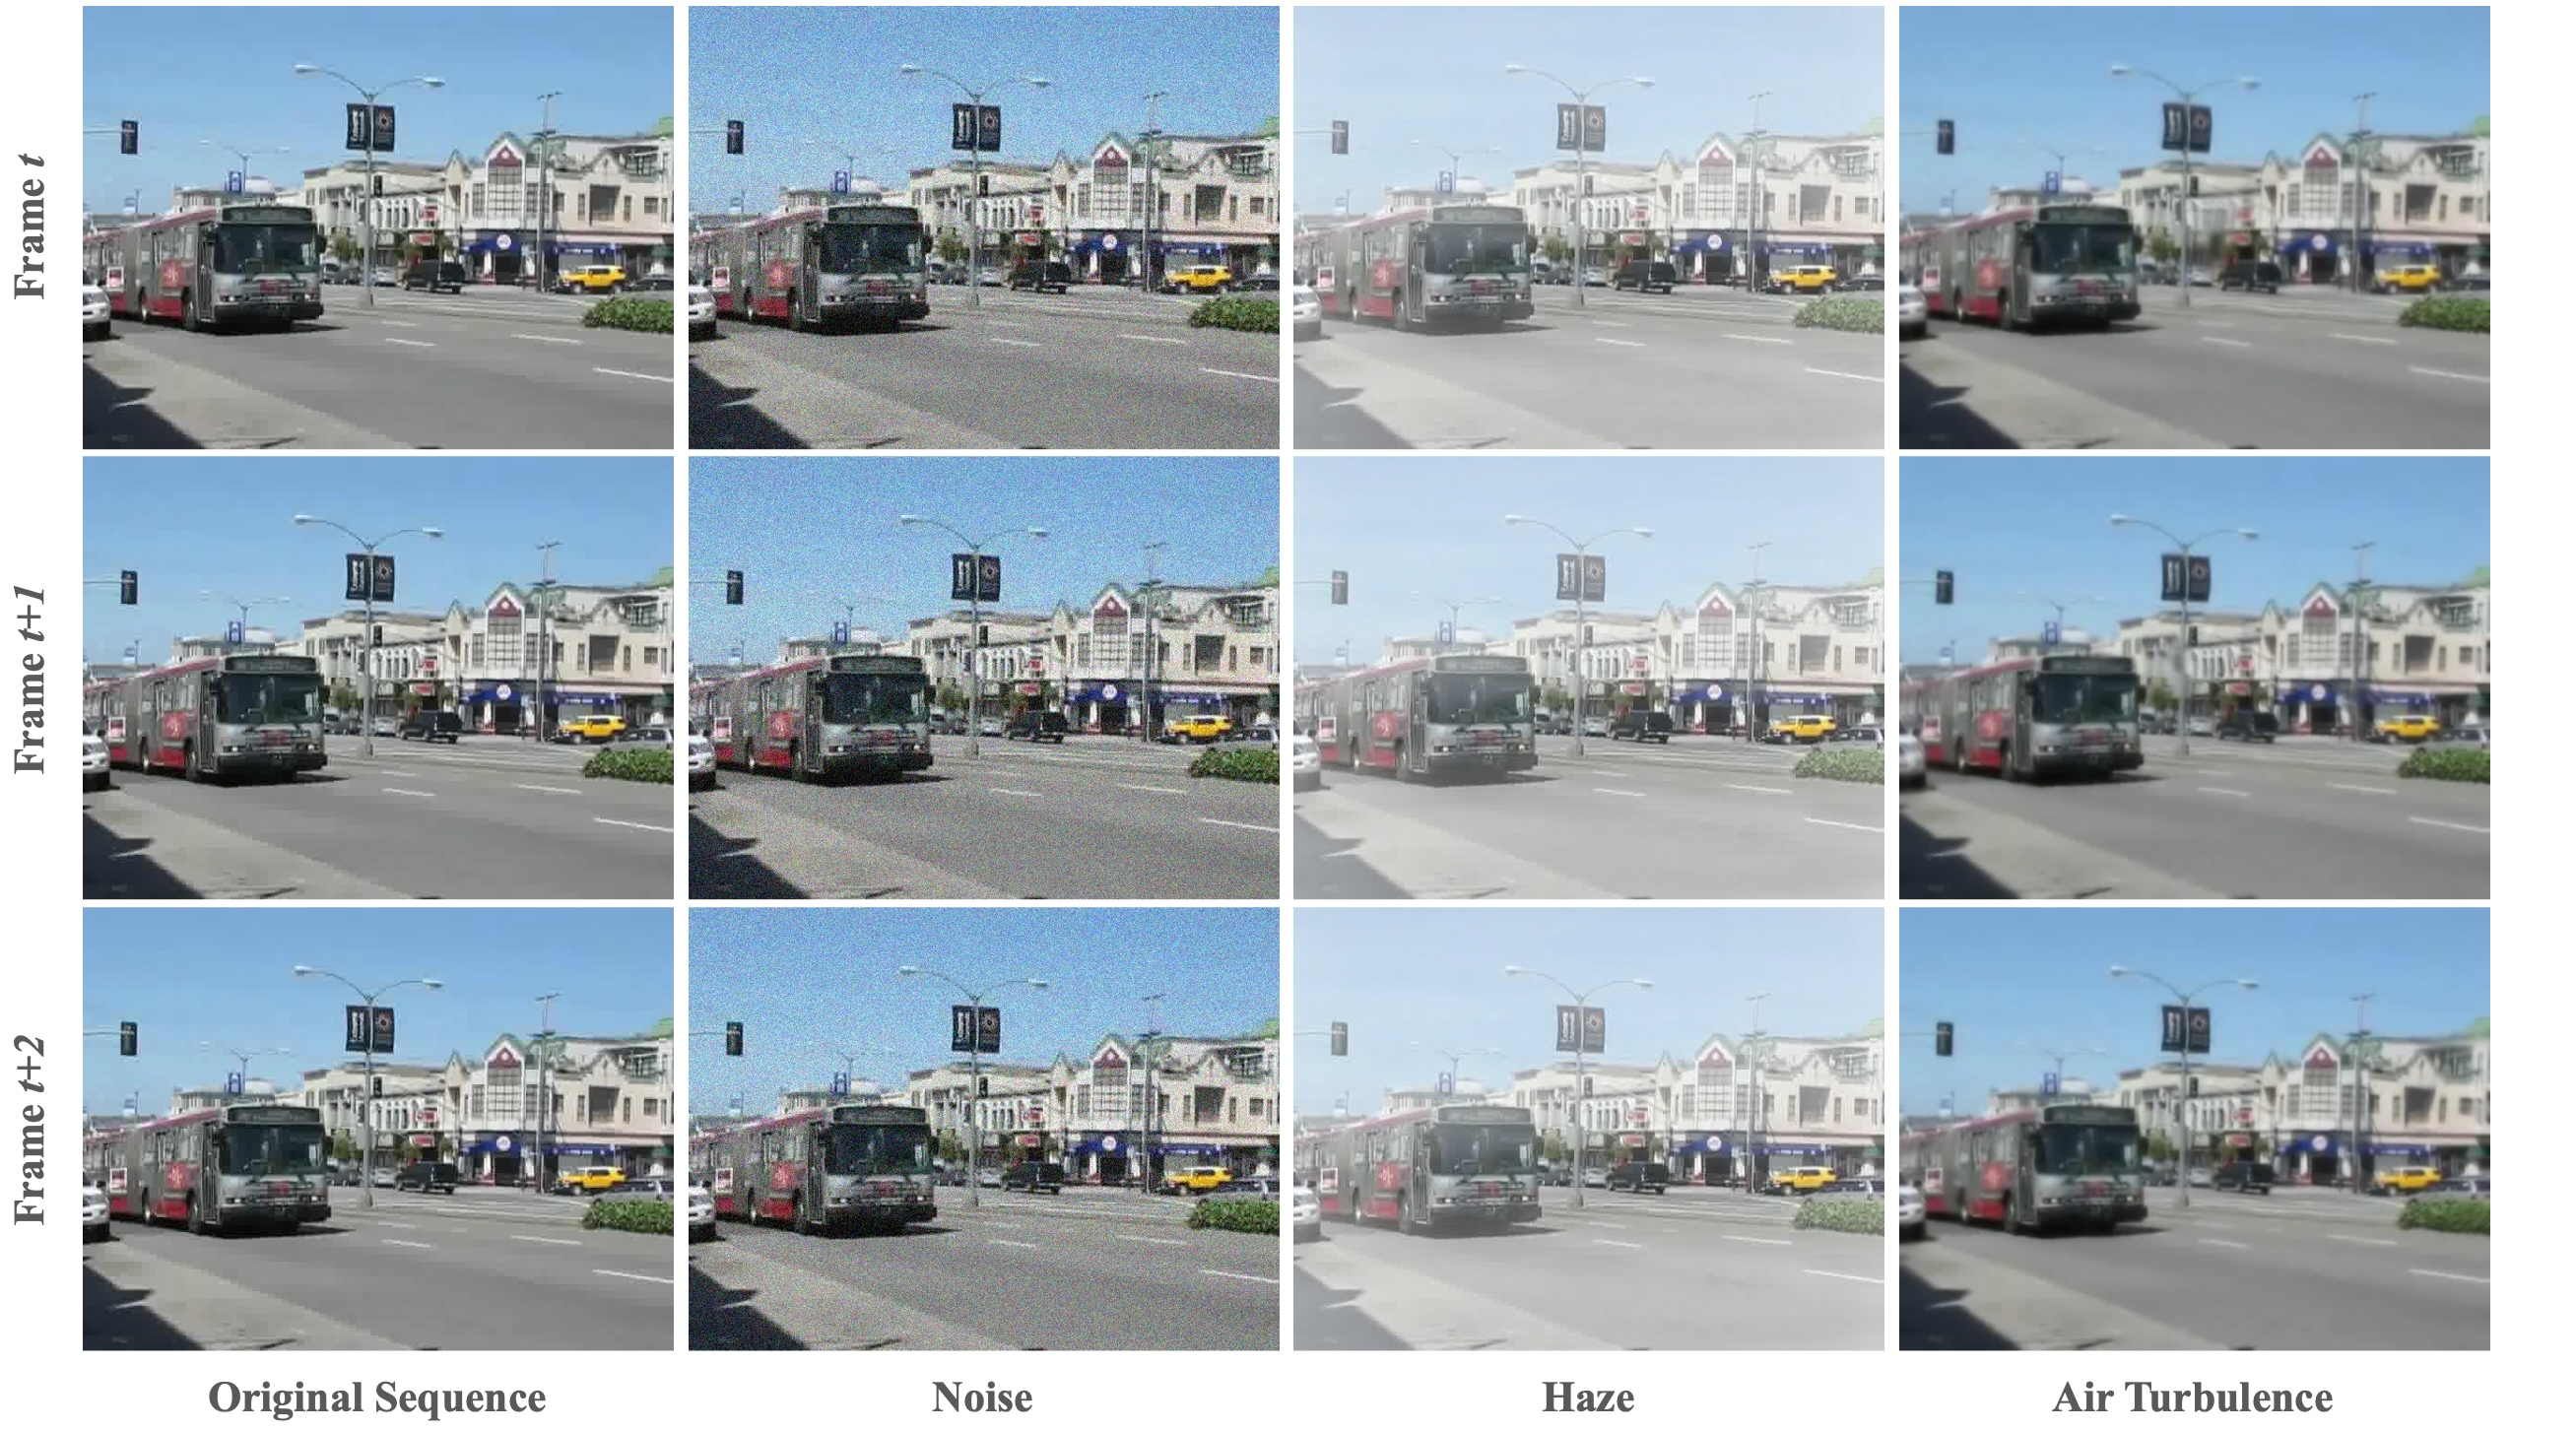
\includegraphics[width = 0.99\linewidth]{figures/test_sample.jpg}
    \caption{A snippet of the ImageNetVOD dataset and three forms of degradation. The original frames are from the testing video \textit{ILSVRC2015\_test\_00028000.mp4} and $t=32$.}
    \label{fig:test_sample}
\end{figure*}

\subsection{Adverse image condition synthesis}
\label{synthesis}
Real-world VOD often faces the challenge of domain gaps caused by adverse image conditions. Because of the complexity of image degradation, testing domain adaptation algorithms under various conditions is desired. However, appropriate datasets for testing the domain adaptation algorithm for VOD models trained on the ImageNetVOD dataset are unavailable. In this work, we synthesized videos in three common imaging conditions: noise, air turbulence, and haze. Each video has its distinct degradation parameter, with the profile varies temporally. A sample image sequence from the original dataset and the associated three degraded sequences are shown in Fig. \ref{fig:test_sample}. The unsupervised property of the algorithm guarantees that our method will be effective in real-world unknown degradations. The simulation of the three adverse image conditions is described below:

\noindent \textbf{Noise.} Noise is the predominant degradation in the low-light conditions. The noise in our experiment is modeled with:
\begin{equation}
    \widetilde{I}(h,w,t) = I(h,w,t) + n(h,w,t),
\end{equation}
\noindent where $I$ is the input image sequence, $\widetilde{I}$ is the degraded image sequence, $h$, $w$, and $t$ are the sequence's height, width, and frame indices. $n(h,w,t)\sim \mathcal{N}(0, \sigma^2)$ is the Gaussian noise. We randomly sample the variance of the noise in $\sigma^2\in [10/255, 50/255]$. Each sequence has its distinct variance.

\noindent \textbf{Air Turbulence.} In long-range imaging conditions, air turbulence may affect the performance of computer vision models significantly \cite{Liu_2024_WACV}. The air turbulence primarily causes random pixel displacement and spatially varying blur on the image \cite{chan2023computational}. We utilized the popular P2S simulator \cite{chimitt2020simulating, Mao_2021_ICCV} to synthesize the degraded video:
\begin{equation}
    \widetilde{I}(h,w,t) = \text{P2S}(I(h,w,t); n(h,w,t)).
\end{equation}
The P2S simulator converts the Gaussian random seed $n$ to spatially varying pixel displacement and blur. Inspired by \cite{chimitt2022real, zhang2022imaging}, we applied the temporal correlation and varying kernel size to improve the diversity and fidelity of the synthetic turbulence. Each image sequence has a distinct turbulence strength and profile.

\noindent \textbf{Haze.} Haze is a crucial adverse image condition in VOD application scenarios, especially in surveillance systems and automated driving. The hazy video can be modeled with the transmission function \cite{cai2016dehazenet}:
\begin{equation}
    \widetilde{I}(h,w,t) = I(h,w,t)e^{-\beta d(h,w,t)} + A(1-e^{-\beta d(h,w,t)} ),
\end{equation}
\noindent where $e^{-\beta d(h,w,t)}$ is the transmission rate, $\beta$ is the scattering coefficient, $A=255$ is the maximum intensity of a pixel, and $d(h,w,t)$ is the relative depth value measured by \cite{Godard_2019_mono}. Like other degradations, each sequence has its own scattering coefficient randomly sampled from a uniform distribution $\beta \in [0.5,1.5]$. 

\begin{table*}
\centering
\setlength{\aboverulesep}{0pt}
\setlength{\belowrulesep}{0pt}
\resizebox{0.99\textwidth}{!}{
\begin{tabular}{l|ccc|ccc|ccc}
\toprule[1pt]
    Degradation & \multicolumn{3}{c|}{Noise} & \multicolumn{3}{c|}{Air Turbulence} & \multicolumn{3}{c}{Haze}   \\
    \hline
    %\cmidrule(lr){1-1} \cmidrule(lr){2-3} \cmidrule(lr){4-5} \cmidrule(lr){6-7}  \cmidrule(lr){8-9}  \cmidrule(lr){10-12} 
Model & YOLOV-S & YOLOV-L & YOLOV-X & YOLOV-S & YOLOV-L & YOLOV-X & YOLOV-S & YOLOV-L & YOLOV-X \\
\hline
Source-only  & 38.0 & 57.0 & 60.4 & 63.2 & 72.7 & 73.9 & 57.2 & 70.7 & 73.0 \\
\hline
PL \textit{w.} SE \cite{li2021free}  & 47.8  & 61.4  & 62.3  & 64.3  & 73.2  & 74.1  & 61.1  & 73.2  & 74.5  \\
\hline
% Naive MT & 56.9  & 71.2  & 71.0  & 64.8  & 74.8  & 75.5  & 67.2  & 76.6  & 78.5  \\
Basic MT & 54.8  & 70.3  & 70.6  & 64.1  & 74.2  & 74.4  & 64.7  & 75.3  & 76.9  \\
STAR-MT   & \textbf{57.6}  & \textbf{71.4}  & \textbf{71.5}  & \textbf{65.2}  & \textbf{75.0}  & \textbf{75.7}  & \textbf{68.1}  & \textbf{78.0}  & \textbf{78.9}  \\
\hline
Oracle    & 61.0  & 72.5  & 72.7  & 66.7  & 76.4  & 78.3  & 69.7  & 79.6  & 80.2  \\
\bottomrule[1pt]
\end{tabular}
}
\caption{Performance comparison on AP50(\%). The larger, the better. ``PL" refers to the pseudo-label method, and ``Source-only” refers to the models trained by only using labeled source domain data.}
\label{table:overall}
\end{table*}

\subsection{Dataset and baselines}
In Section \ref{synthesis}, for each degradation type identified, we generated a corresponding synthetic target-domain dataset utilizing the ImageNetVID dataset \cite{russakovsky2015imagenet} as the source. Comprising 30 classes set against diverse natural backdrops, ImageNetVID provides over 1 million training frames and more than 100,000 validation frames. We used all frames from this source dataset to synthesize the target-domain datasets. Consequently, each domain can retain the same set of labels. Fig \ref{fig:effect} shows a snippet of the testing set of our synthetic degradations, along with the visualization of the detection results before and after the domain adaptation. The visual comparison proves the efficacy of the proposed method.

\begin{figure*}[t]
\small
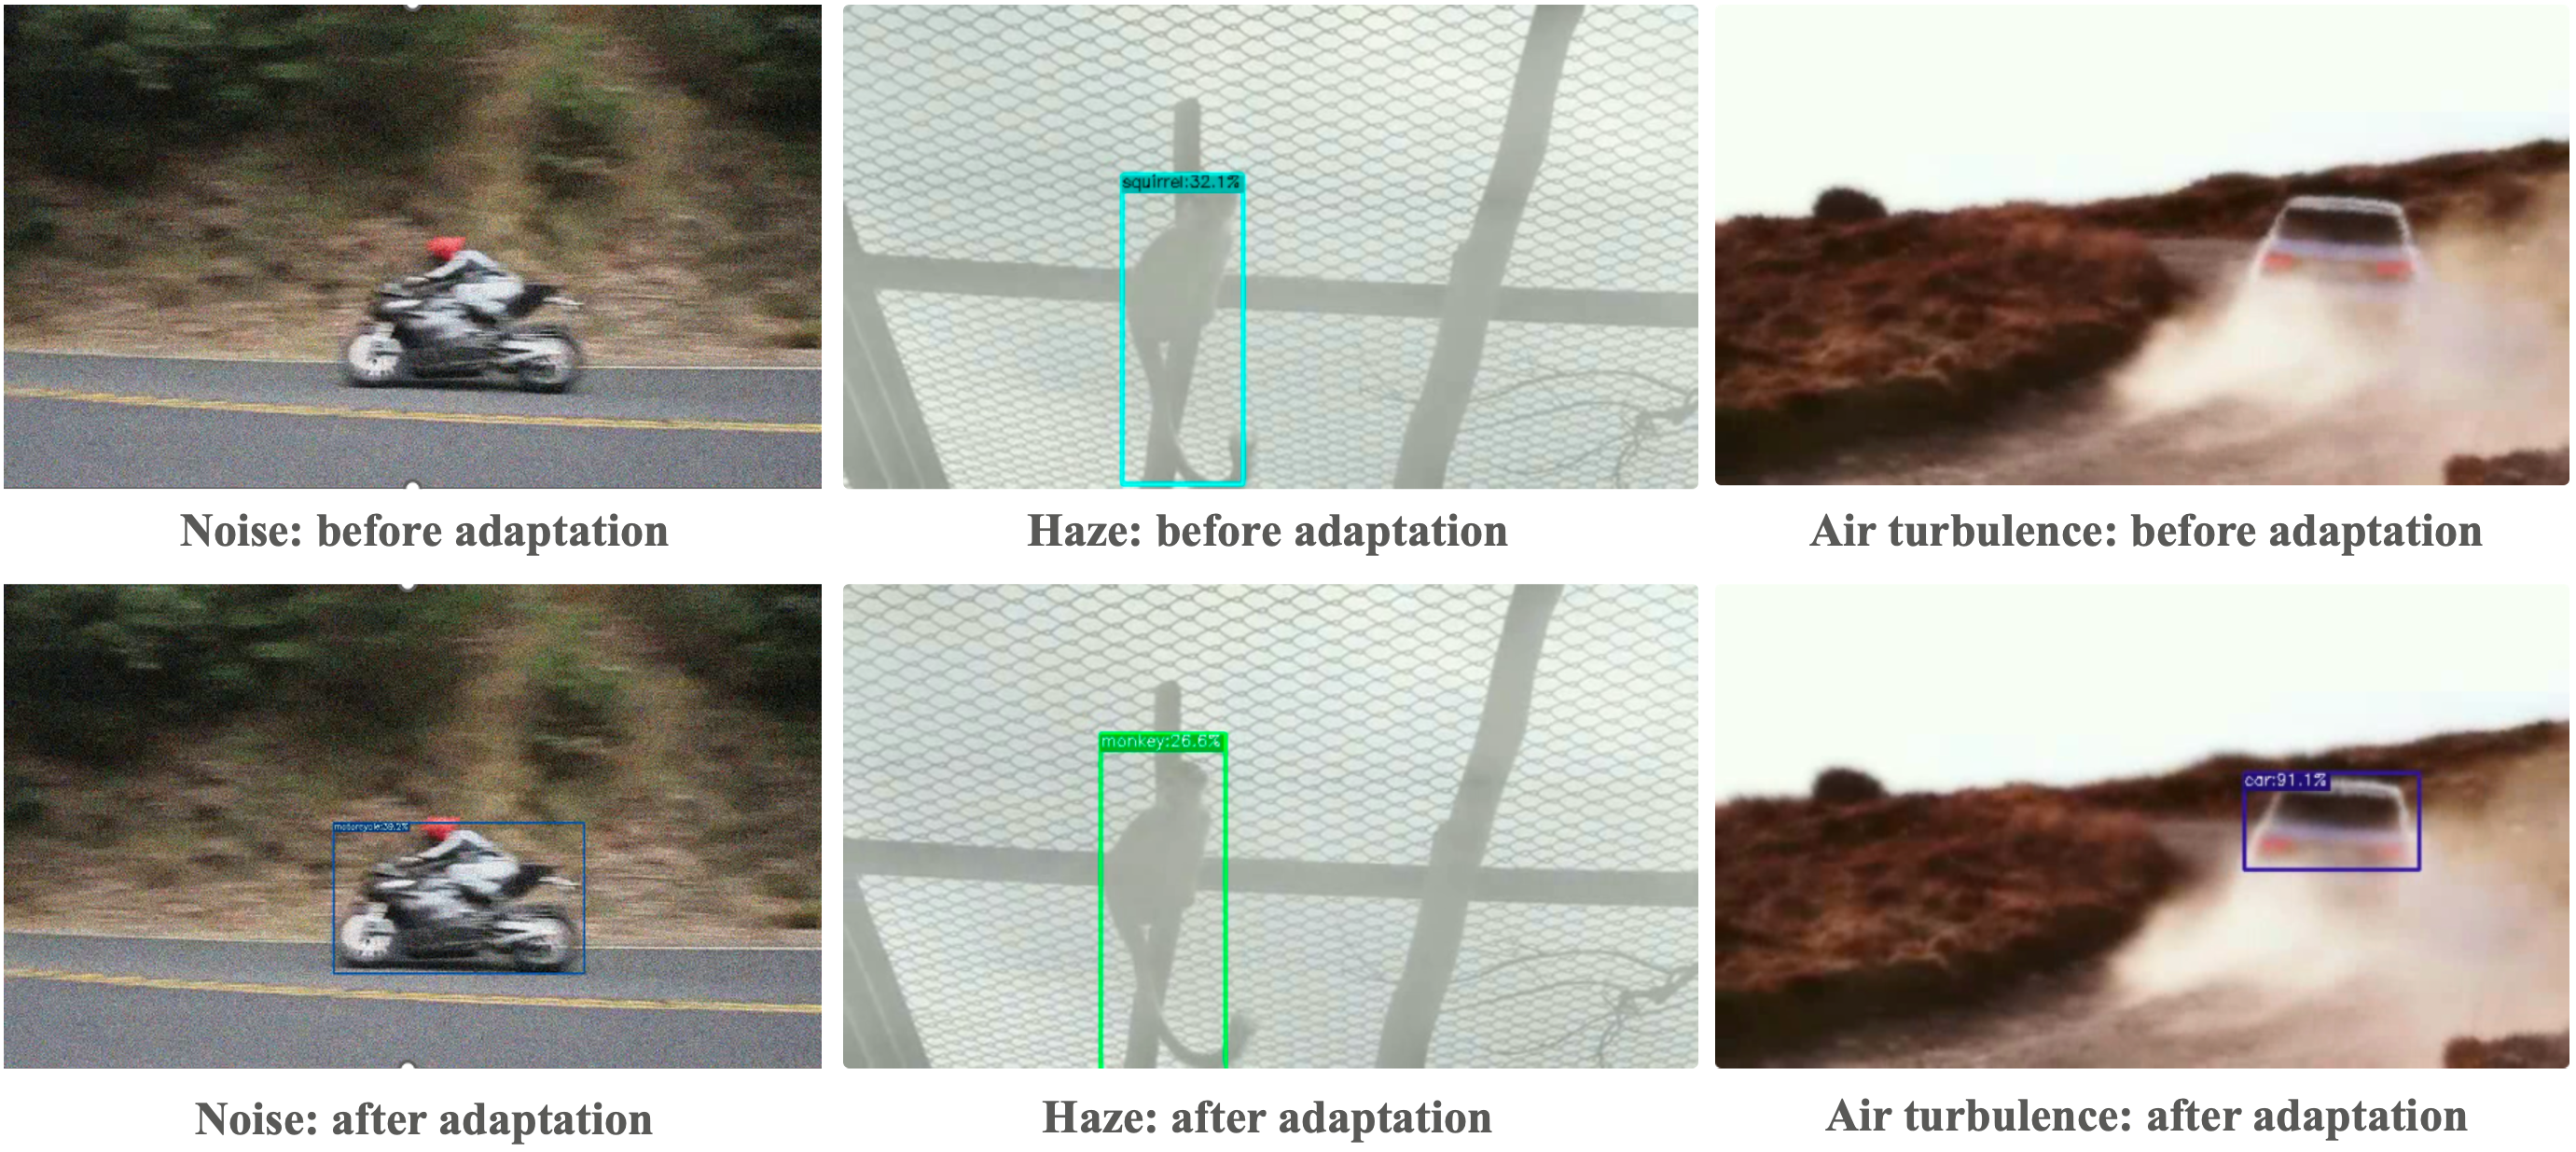
\includegraphics[width=\linewidth]{figures/effect.png}%
\caption{Visual comparison before and after the SFDA by STAR-MT. All experiments are conducted with YOLOV-S.}
\label{fig:effect}
\end{figure*}

Following its publicly available codebase, we trained the YOLOV in all three scales — small (S), large (L), and extra-large (X) — using the source dataset. In our experiment, the post-processing method was omitted as it does not pertain to our algorithms. These models were then directly tested on target domains, with the findings detailed in Table \ref{table:overall}. The Average Precision at $50\%$ threshold (AP50) on the source domain is registered as $77.3\%$, $83.6\%$, and $85.0\%$ for YOLOV-S, YOLOV-L, and YOLOV-X, respectively. The significant degradation in performance, when we test the source-train model on the target domain dataset, indicates that challenging image conditions markedly reduce the performance of the VOD models.

In addition to the initial training, we used a supervised approach to fine-tune the source-trained YOLOV models on the target domain datasets. This supervised fine-tuning serves as a theoretical benchmark for the upper limit of performance achievable through unsupervised adaptation. Deviating from the original pipeline, which involves training the base detector prior to the temporal aggregation module, we discovered that directly fine-tuning the temporal aggregation module leads to improved outcomes. Therefore, our fine-tuning focuses solely on the temporal aggregation module for the target domains, as detailed in \cite{shi2023yolov}. The results of this supervised fine-tuning, labeled as ``oracle", are also presented in Table \ref{table:overall}.

Before implementing the mean-teacher-based methods, we conducted a preliminary experiment with the pseudo-label (PL) algorithm. In this approach, models trained on the source domain are employed to process all videos in the target domain's training set, generating initial predictions. They are then filtered by threshold 0.5 on the product of objectiveness and the maximal class scores to generate pseudo labels. Since fine-tuning the single-frame backbone always causes catastrophic failure, we fixed the parameters in the backbone module and only trained the temporal aggregation module with pseudo labels. After training, we utilized the self-entropy \cite{li2021free} as the indicator to select the potential best model. The result is also demonstrated in Table \ref{table:overall}.

\subsection{Implementation details of STAR-MT}
Adhering closely to the YOLOV codebase, we maintained most of the original settings unaltered. For hyperparameter configuration, we empirically set the teacher model's smoothing coefficient, $\alpha$, to 0.9995 and the weighting factor, $\gamma$, of the $\mathcal{L}_{cls}$ to 0.2. The model training was executed using Stochastic Gradient Descent (SGD) with a batch size of 1 over 10,000 iterations. We initialized the learning rate at $2 \times 10^{-4}$ and applied a cosine annealing scheduler, tapering it down to $1 \times 10^{-4}$. In the evaluation phase, only the teacher model was utilized for inference. The mean Average Precision (mAP) was calculated with an IoU threshold of 0.5. All experiments are conducted on NVIDIA 3080 Ti and V100 GPUs.

\begin{figure}[t]
\small
\begin{minipage}[b]{.49\linewidth}
  \centering
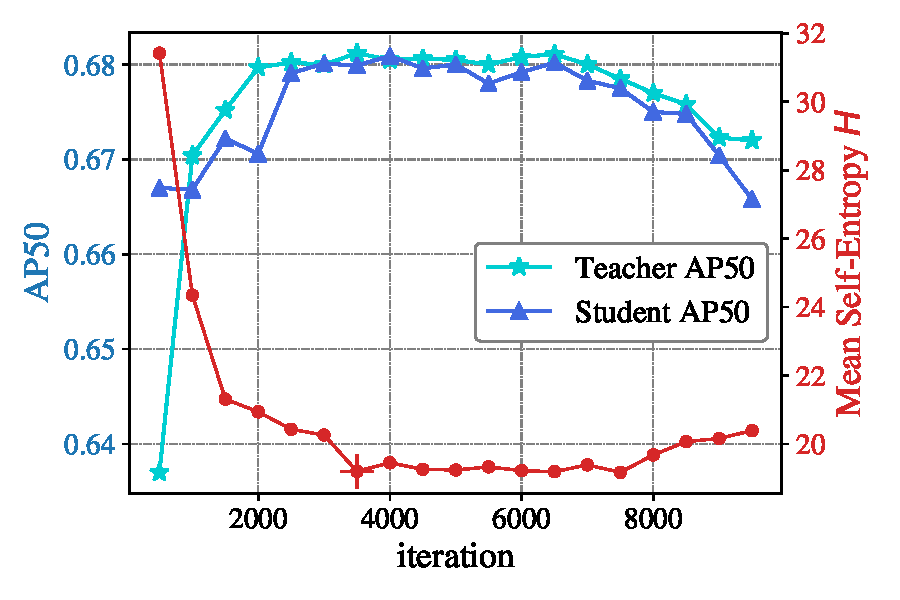
\includegraphics[width=\linewidth]{figures/yolovs.pdf}%
  \vspace{0.1cm}
  \centerline{(a) YOLOV-S}
\end{minipage}
\hfill
\begin{minipage}[b]{0.49\linewidth}
  \centering
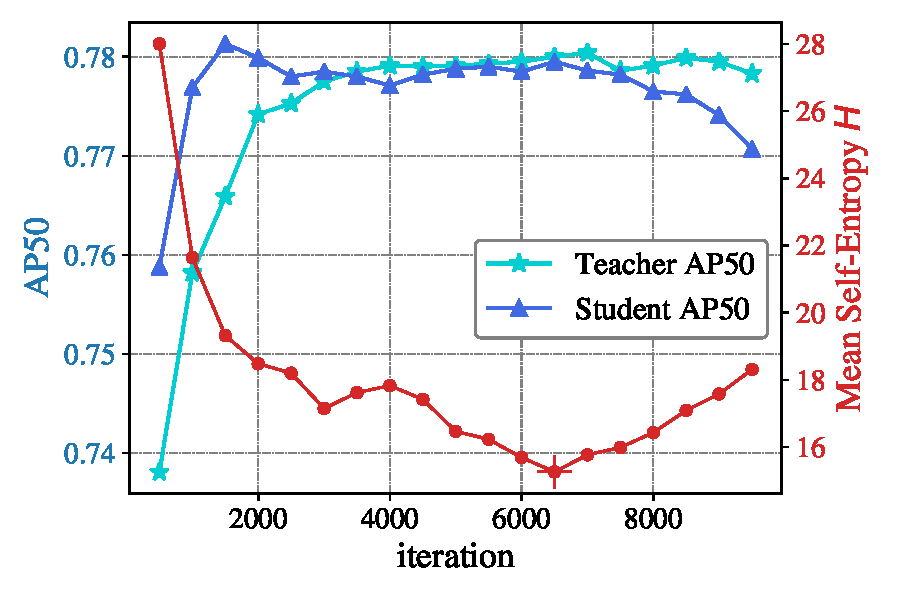
\includegraphics[width=\linewidth]{figures/yolovl.pdf}%
  \vspace{0.1cm}
  \centerline{(b) YOLOV-L}
\end{minipage}
\caption{The teacher model's AP50 and mean self-entropy $H$ variation in the STAR-MT training of YOLOV-S and YOLOV-L. Both experiments are conducted on clean $\rightarrow$ haze. The $H$ indicating the best teacher model are marked in the figures with ``\textcolor{red}{+}".}
\label{fig:curve}
\end{figure}

For each sequence in our domain adaptation experiments, 32 frames are loaded. Mosaic augmentation was disabled for all these experiments. However, we have retained both random flip and perspective transformations, applying these consistently to both weakly and strongly augmented sequence pairs. The key distinction between weak and strong augmentation lies in the strength of random chromatic transformation. Random erasing is involved only in the strong augmentation. In the TRS, random masking is applied to restrict the temporal information the student model can access, compelling it to enhance the temporal aggregation capability. The masking rate is $r\%$ where $r$ is randomly sampled from $[0, 75]$.

The performance of the STAR-MT method is demonstrated in Table \ref{table:overall}. Our method shows a significant improvement in the SFDA for VOD under all three adverse image conditions. It also demonstrates a clear advantage over conventional methods like pseudo-labeling and basic mean-teacher learning. Notably, although the method seems straightforward and not complicated, \textit{the performance of our method closely approaches that of supervised fine-tuning}. To illustrate the correlation between mean self-entropy $H$ and the performance of SFDA, we drew the variations in model performance alongside the change in $H$ value on the evaluation set, as shown in Fig \ref{fig:curve}. The $H$ values were calculated using a sliding window average over 100 iterations. We can observe the lowest value of $H$ aligns well with the peak performance of the model.


\subsection{Ablation study}
\noindent \textbf{Efficacy of alternate refinement.} One major novelty in this paper is the spatial refinement stage, as an alternately updated module in addition to the normal mean teacher learning framework. The key insights behind this are 1) temporally enhanced features of the teacher model can be used to generate reliable pseudo labels for the training of the single-frame detection head, and 2) training the single-frame detection head under the YOLOV setting is suboptimal. Thus, it needs additional guidance. From the comparison between the basic mean-teacher method (TRS only) and the proposed STAR-MT in Table \ref{table:overall}, we can verify the efficacy of alternate refinement with the spatial refinement stage. To demonstrate that the pseudo labels from the YOLOV are of higher quality, we conducted source-free domain adaptation for the YOLOX. We follow the mean-teacher framework and use the pseudo labels generated by YOLOX and YOLOV to guide the training of the student network. The result is shown in Table \ref{tab:SRS}. The model guided by the temporally refined labels in YOLOV gets better performance, which provides evidence for the efficacy of SRS.

% \noindent \textbf{Effectiveness of weight initialization for the student model.} The teacher
% model serves as a performance lower bound for the student model \cite{liu2023periodically}. Observing that the performance of teacher model is better than the student model in most iterations, we update the weight of the student model by that of the teacher model in the beginning of each stage. We evaluate the effect in Table, which 
\begin{table}
    \centering
    \begin{tabular}{l|c|c}
    \hline
        Model & YOLOX-S &  YOLOX-L  \\
        \hline
        Source-only  & 35.9 & 56.6  \\
        PL guided by YOLOX  & 49.2 & 61.3  \\
        PL guided by YOLOV & 51.0 & 62.9\\
        \hline 
        Oracle & 56.7 & 66.0 \\
    \hline
    \end{tabular}
    \caption{The efficacy of YOLOV as the teacher model for the SFDA of the single-frame detection backbone. All experiments are conducted on clean $\rightarrow$ noise. The metric is AP50(\%), the larger, the better.}
    \label{tab:SRS}
\end{table}


\begin{table}
    \centering
    \begin{tabular}{c|c|c|c|c}
    \hline
        $\mathcal{L}_{MSE}$ & $\mathcal{L}_{BCE}$ & $\mathcal{L}_{cls}$ & YOLOV-S  & YOLOV-L \\
        \hline
        \xmark & \cmark & \cmark & 62.1 & 71.5 \\
        \cmark & \cmark & \xmark & 67.6 & 77.4 \\
        \cmark & \xmark & \cmark & 67.8 & 77.3 \\
        \cmark & \cmark & \cmark & \textbf{68.1} & \textbf{78.0} \\
    \hline
    \end{tabular}
    \caption{The efficacy of losses. All experiments are conducted on clean $\rightarrow$ haze. The metric is AP50(\%), the larger, the better.}
    \label{tab:losses}
\end{table}

\noindent \textbf{Efficacy of losses.} In our study, the three utilized loss functions are categorized as feature alignment loss $\mathcal{L}_{MSE}$ and pseudo-label based losses ($\mathcal{L}_{BCE}$ and $\mathcal{L}_{cls}$). We experimented with various reasonable combinations of these loss terms to assess their impact. In all combinations, at least one pseudo-label-based loss was maintained. The results are detailed in Table \ref{tab:losses}. Initially, we excluded the feature alignment loss $\mathcal{L}_{MSE}$ and observed a significant decline in adaptation performance. This indicates the model's high sensitivity to label quality and the importance of restricting the feature space generated by the detection head. Further, we excluded $\mathcal{L}_{MSE}$ and $\mathcal{L}_{cls}$ separately to evaluate their individual contributions. The results confirmed the effectiveness of both losses.

\begin{table}
    \centering
    \begin{tabular}{c|c|c|c|c}
    \hline
        Model & $\tau = 50$ & $\tau = 100$ & $\tau = 200$  & $\tau = 500$ \\
        \hline
        YOLOV-S & 68.0 & \textbf{68.1} & 67.6 & 67.8 \\
        YOLOV-L & 76.9 & 77.5 & \textbf{78.0} & 77.7 \\
        YOLOV-X & 78.2 & 78.4 & \textbf{78.9} & 78.8 \\
    \hline
    \end{tabular}
    \caption{The impact of the number of iterations in each stage. All experiments are conducted on clean $\rightarrow$ haze. The metric is AP50(\%), the larger, the better.}
    \label{tab:iteration}
\end{table}

\noindent \textbf{Number of iterations for each stage.} We also evaluated the optimal number of fine-tuning iterations, $\tau$, for each stage within a period. For this purpose, we conducted experiments that set $\tau$ to various values: 50, 100, 200, and 500, while maintaining 10,000 training iterations. The determination of optimal results within this range was based on the mean self-entropy $H$ values, where the teacher model associated with the first local minima of $H$ is selected. This assessment was carried out across all three model scales, and the findings are presented in Table \ref{tab:iteration}. The results indicate that different scales of the model may require distinct hyperparameters to achieve optimal adaptation performance.
\section{Conclusion}

In this paper, we propose a pioneering approach to explore the source-free domain adaptation (SFDA) for video object detection (VOD). Specifically, we developed a novel SFDA method for a one-stage-based detector, YOLOV. The proposed STAR-MT technique significantly improves the performance of the video object detector in adverse image conditions without access to the target domain label or source domain data. Owing to its unsupervised nature, this work can be seamlessly applied to real-world scenarios requiring VOD models. The proposed method could serve as a baseline for future research in unsupervised domain adaptation for video object detection. 




\section{Acknowledgment}
Futurewei Technologies Inc. funded this research while the
first author was an intern there. We are grateful to the company’s
IC Lab for the research assistance.


{
    \small
    \bibliographystyle{ieeenat_fullname}
    \bibliography{main}
}

% WARNING: do not forget to delete the supplementary pages from your submission 
% \clearpage
\setcounter{page}{1}
\maketitlesupplementary


\section{Rationale}
\label{sec:rationale}
% 
Having the supplementary compiled together with the main paper means that:
% 
\begin{itemize}
\item The supplementary can back-reference sections of the main paper, for example, we can refer to \cref{sec:intro};
\item The main paper can forward reference sub-sections within the supplementary explicitly (e.g. referring to a particular experiment); 
\item When submitted to arXiv, the supplementary will already included at the end of the paper.
\end{itemize}
% 
To split the supplementary pages from the main paper, you can use \href{https://support.apple.com/en-ca/guide/preview/prvw11793/mac#:~:text=Delete%20a%20page%20from%20a,or%20choose%20Edit%20%3E%20Delete).}{Preview (on macOS)}, \href{https://www.adobe.com/acrobat/how-to/delete-pages-from-pdf.html#:~:text=Choose%20%E2%80%9CTools%E2%80%9D%20%3E%20%E2%80%9COrganize,or%20pages%20from%20the%20file.}{Adobe Acrobat} (on all OSs), as well as \href{https://superuser.com/questions/517986/is-it-possible-to-delete-some-pages-of-a-pdf-document}{command line tools}.

\end{document}
